% xcolor and define colors -------------------------
\usepackage{xcolor}

% https://www.viget.com/articles/color-contrast/
\definecolor{purple}{HTML}{5601A4}
\definecolor{navy}{HTML}{0D3D56}
\definecolor{ruby}{HTML}{9a2515}
\definecolor{alice}{HTML}{107895}
\definecolor{daisy}{HTML}{EBC944}
\definecolor{coral}{HTML}{F26D21}
\definecolor{kelly}{HTML}{829356}
\definecolor{cranberry}{HTML}{E64173}
\definecolor{jet}{HTML}{131516}
\definecolor{asher}{HTML}{555F61}
\definecolor{slate}{HTML}{314F4F}

% Mixtape Sessions
\definecolor{picton-blue}{HTML}{00b7ff}
\definecolor{violet-red}{HTML}{ff3881}
\definecolor{sun}{HTML}{ffaf18}
\definecolor{electric-violet}{HTML}{871EFF}

\newcommand\pictonBlue[1]{{\color{picton-blue}#1}}
\newcommand\sun[1]{{\color{sun}#1}}
\newcommand\electricViolet[1]{{\color{electric-violet}#1}}
\newcommand\violetRed[1]{{\color{violet-red}#1}}

\newcommand\bgPictonBlue[1]{{\colorbox{picton-blue!20!white}{#1}}}
\newcommand\bgSun[1]{{\colorbox{sun!20!white}{#1}}}
\newcommand\bgElectricViolet[1]{{\colorbox{electric-violet!20!white}{#1}}}
\newcommand\bgVioletRed[1]{{\colorbox{violet-red!20!white}{#1}}}

\def\code#1{\texttt{#1}}

% Main theme colors
\definecolor{accent}{HTML}{00b7ff}
\definecolor{accent2}{HTML}{871EFF}
\definecolor{gray100}{HTML}{f3f4f6}
\definecolor{gray800}{HTML}{1F292D}


% Beamer Options -------------------------------------

% Background
\setbeamercolor{background canvas}{bg = white}

% Change text margins
\setbeamersize{text margin left = 15pt, text margin right = 15pt} 

% \alert
\setbeamercolor{alerted text}{fg = accent2}

% Frame title
\setbeamercolor{frametitle}{bg = white, fg = jet}
\setbeamercolor{framesubtitle}{bg = white, fg = accent}
\setbeamerfont{framesubtitle}{size = \small, shape = \itshape}

% Block
\setbeamercolor{block title}{fg = white, bg = accent2}
\setbeamercolor{block body}{fg = gray800, bg = gray100}

% Title page
\setbeamercolor{title}{fg = gray800}
\setbeamercolor{subtitle}{fg = accent}

%% Custom \maketitle and \titlepage
\setbeamertemplate{title page}
{
    %\begin{centering}
        \vspace{20mm}
        {\Large \usebeamerfont{title}\usebeamercolor[fg]{title}\inserttitle}\\
        {\large \itshape \usebeamerfont{subtitle}\usebeamercolor[fg]{subtitle}\insertsubtitle}\\ \vspace{10mm}
        {\insertauthor}\\
        {\color{asher}\small{\insertdate}}\\
    %\end{centering}
}

% Table of Contents
\setbeamercolor{section in toc}{fg = accent!70!jet}
\setbeamercolor{subsection in toc}{fg = jet}

% Button 
\setbeamercolor{button}{bg = accent}

% Remove navigation symbols
\setbeamertemplate{navigation symbols}{}

% Table and Figure captions
\setbeamercolor{caption}{fg=jet!70!white}
\setbeamercolor{caption name}{fg=jet}
\setbeamerfont{caption name}{shape = \itshape}

% Bullet points

%% Fix spacing between items
\let\olditemize=\itemize 
\let\endolditemize=\enditemize 
\renewenvironment{itemize}{\vspace{0.25em}\olditemize \itemsep0.25em}{\endolditemize}

%% Fix left-margins
\settowidth{\leftmargini}{\usebeamertemplate{itemize item}}
\addtolength{\leftmargini}{\labelsep}

%% enumerate item color
\setbeamercolor{enumerate item}{fg = accent}
\setbeamerfont{enumerate item}{size = \small}
\setbeamertemplate{enumerate item}{\insertenumlabel.}

%% itemize
\setbeamercolor{itemize item}{fg = accent!70!white}
\setbeamerfont{itemize item}{size = \small}
\setbeamertemplate{itemize item}[circle]

%% right arrow for subitems
\setbeamercolor{itemize subitem}{fg = accent!60!white}
\setbeamerfont{itemize subitem}{size = \small}
\setbeamertemplate{itemize subitem}{$\rightarrow$}

\setbeamertemplate{itemize subsubitem}[square]
\setbeamercolor{itemize subsubitem}{fg = jet}
\setbeamerfont{itemize subsubitem}{size = \small}








% Links ----------------------------------------------

\usepackage{hyperref}
\hypersetup{
  colorlinks = true,
  linkcolor = accent2,
  filecolor = accent2,
  urlcolor = accent2,
  citecolor = accent2,
}


% Line spacing --------------------------------------
\usepackage{setspace}
\setstretch{1.35}


% \begin{columns} -----------------------------------
\usepackage{multicol}


% Fonts ---------------------------------------------
% Beamer Option to use custom fonts
\usefonttheme{professionalfonts}

% \usepackage[utopia, smallerops, varg]{newtxmath}
% \usepackage{utopia}
\usepackage[sfdefault,light]{roboto}

% Small adjustments to text kerning
\usepackage{microtype}



% Remove annoying over-full box warnings -----------
\vfuzz2pt 
\hfuzz2pt


% Table of Contents with Sections
\setbeamerfont{myTOC}{series=\bfseries, size=\Large}
\AtBeginSection[]{
        \frame{
            \frametitle{Roadmap}
            \tableofcontents[current]   
        }
    }


% Tables -------------------------------------------
% Tables too big
% \begin{adjustbox}{width = 1.2\textwidth, center}
\usepackage{adjustbox}
\usepackage{array}
\usepackage{threeparttable, booktabs, adjustbox}
    
% Fix \input with tables
% \input fails when \\ is at end of external .tex file
\makeatletter
\let\input\@@input
\makeatother

% Tables too narrow
% \begin{tabularx}{\linewidth}{cols}
% col-types: X - center, L - left, R -right
% Relative scale: >{\hsize=.8\hsize}X/L/R
\usepackage{tabularx}
\newcolumntype{L}{>{\raggedright\arraybackslash}X}
\newcolumntype{R}{>{\raggedleft\arraybackslash}X}
\newcolumntype{C}{>{\centering\arraybackslash}X}

% Figures

% \imageframe{img_name} -----------------------------
% from https://github.com/mattjetwell/cousteau
\newcommand{\imageframe}[1]{%
    \begin{frame}[plain]
        \begin{tikzpicture}[remember picture, overlay]
            \node[at = (current page.center), xshift = 0cm] (cover) {%
                \includegraphics[keepaspectratio, width=\paperwidth, height=\paperheight]{#1}
            };
        \end{tikzpicture}
    \end{frame}%
}

% subfigures
\usepackage{subfigure}


% Highlight slide -----------------------------------
% \begin{transitionframe} Text \end{transitionframe}
% from paulgp's beamer tips
\newenvironment{transitionframe}{
    \setbeamercolor{background canvas}{bg=accent!40!black}
    \begin{frame}\color{accent!10!white}\LARGE\centering
}{
    \end{frame}
}


% Table Highlighting --------------------------------
% Create top-left and bottom-right markets in tabular cells with a unique matching id and these commands will outline those cells
\usepackage[beamer,customcolors]{hf-tikz}
\usetikzlibrary{calc}
\usetikzlibrary{fit,shapes.misc}

% To set the hypothesis highlighting boxes red.
\newcommand\marktopleft[1]{%
    \tikz[overlay,remember picture] 
        \node (marker-#1-a) at (0,1.5ex) {};%
}
\newcommand\markbottomright[1]{%
    \tikz[overlay,remember picture] 
        \node (marker-#1-b) at (0,0) {};%
    \tikz[accent!80!jet, ultra thick, overlay, remember picture, inner sep=4pt]
        \node[draw, rectangle, fit=(marker-#1-a.center) (marker-#1-b.center)] {};%
}


% DAGS ----------------------------------------------
\usepackage{tikz}
\usetikzlibrary{shapes,decorations,arrows,calc,arrows.meta,fit,positioning}
% Tikz settings optimized for causal graphs.
\tikzset{
    -Latex,auto,node distance =1 cm and 1 cm,semithick,
    state/.style ={ellipse, draw, minimum width = 0.7 cm},
    point/.style = {circle, draw, inner sep=0.04cm,fill,node contents={}},
    bidirected/.style={Latex-Latex,dashed},
    el/.style = {inner sep=2pt, align=left, sloped}
}


% Beamer tricks -------------------------------------
% Make \pause work in align environments
\makeatletter
\renewrobustcmd{\beamer@@pause}[1][]{%
  \unless\ifmeasuring@%
  \ifblank{#1}%
    {\stepcounter{beamerpauses}}%
    {\setcounter{beamerpauses}{#1}}%
  \onslide<\value{beamerpauses}->\relax%
  \fi%
}
\makeatother


\title [Nonparametrics]{Nonparametrics and Local Methods: Nearest Neighbor Methods}
\author{C.Conlon}
\institute{Applied Econometrics}
\date{\today}
\setbeamerfont{equation}{size=\tiny}
\begin{document}

\begin{frame}
\titlepage
\end{frame}

\begin{frame}{Bias Variance Decomposition}
We can decompose any estimator into two components
\begin{align*}
\underbrace{\E[(y- \hat{f}(x))^2]}_{MSE} =\underbrace{\left( \E[\hat{f}(x) - f(x)] \right)^2}_{Bias^2}  +  \underbrace{\E \left[ \left(\hat{f}(x) -\E[\hat{f}(x) \right] \right)^2}_{Variance} 
\end{align*}
\begin{itemize}
\item In general we face a tradeoff between bias and variance.
\item More complicated models reduce \alert{bias}, but at the expense of higher \alert{variance}.
%\item In k-NN as $k$ gets large we reduce the variance (each point has less influence) but we increase the bias since we start incorporating far away and potentially irrelevant information.
%\item In OLS we minimize the variance among unbiased estimators assuming that the true $f$ is linear.
\end{itemize}
\end{frame}

\begin{frame}{Bias Variance Decomposition}
What minimizes MSE?
\begin{align*}
f(x_i) = \E[Y_i | X_i] 
\end{align*}
\begin{itemize}
\item Seems simple enough (but we are back where we started).
\item How do we compute the expectation ?
\begin{itemize}
\item OLS uses entire dataset and adds structure $ y = x \beta$ to the problem.
\item Can use polynomials in $x$.
\item k-NN tries to use local information to estimate conditional mean
\end{itemize}
\end{itemize}
\end{frame}



\begin{frame}{How about logit?}
We write:
\begin{align*}
\E[Y_i | X_i] &= Pr(Y_i =1 | X_i) = p(x_i)\\
 Pr(Y_i =1 | X_i)  &= \frac{1}{1+\exp^{\beta_0 + \beta_1 x_1 + \beta_2 x_2 + \ldots}}
\end{align*}
Or with the log odds transformation:
\begin{align*}
\log \left(\frac{p}{1-p} \right) =\beta_0 + \beta_1 x_1 + \beta_2 x_2 + \ldots
\end{align*}
Logit is \alert{linear} again (in parameters). This is a \alert{generalized linear model}.
\end{frame}

\begin{frame}{How else might we estimate $\E[Y_i | X_i]$?}
Obvious approach:
\begin{itemize}
\item With enough data: look at all values for $X_i = x$ and take the mean.
\item Easy if $X$ is discrete or doesn't take on too many values (Gender, State/Country).
\item Could work if $X$ is continuous but rounded (test scores, years of school, etc.).
\item We could cut $x_i$ into distinct bins (like a histogram).
\end{itemize}
\end{frame}


\begin{frame}{A Fake Data Example}
Following the THF textbook example, we can generate some fake data and let: 
\begin{eqnarray*}
Y=&ORANGE \mbox{ if } Y^{*} &> 0.5 \\
Y=&BLUE  \mbox{ if }   Y^{*} &\leq 0.5
\end{eqnarray*}
\begin{itemize}
\item Easiest way to recover $Y^{*}$ is by running OLS on the linear probability model.
\item Draws from bivariate normal distribution with uncorrelated components but different means (2 overlapping types)
\item Mixture of 10 low variance (nearly point mass) normal distributions where the individual means were drawn from another normal distribution. (10 nearly distinct types).
\end{itemize}
\end{frame}

\begin{frame}{Linear Probability Model}
\begin{figure}[htbp]
\begin{center}
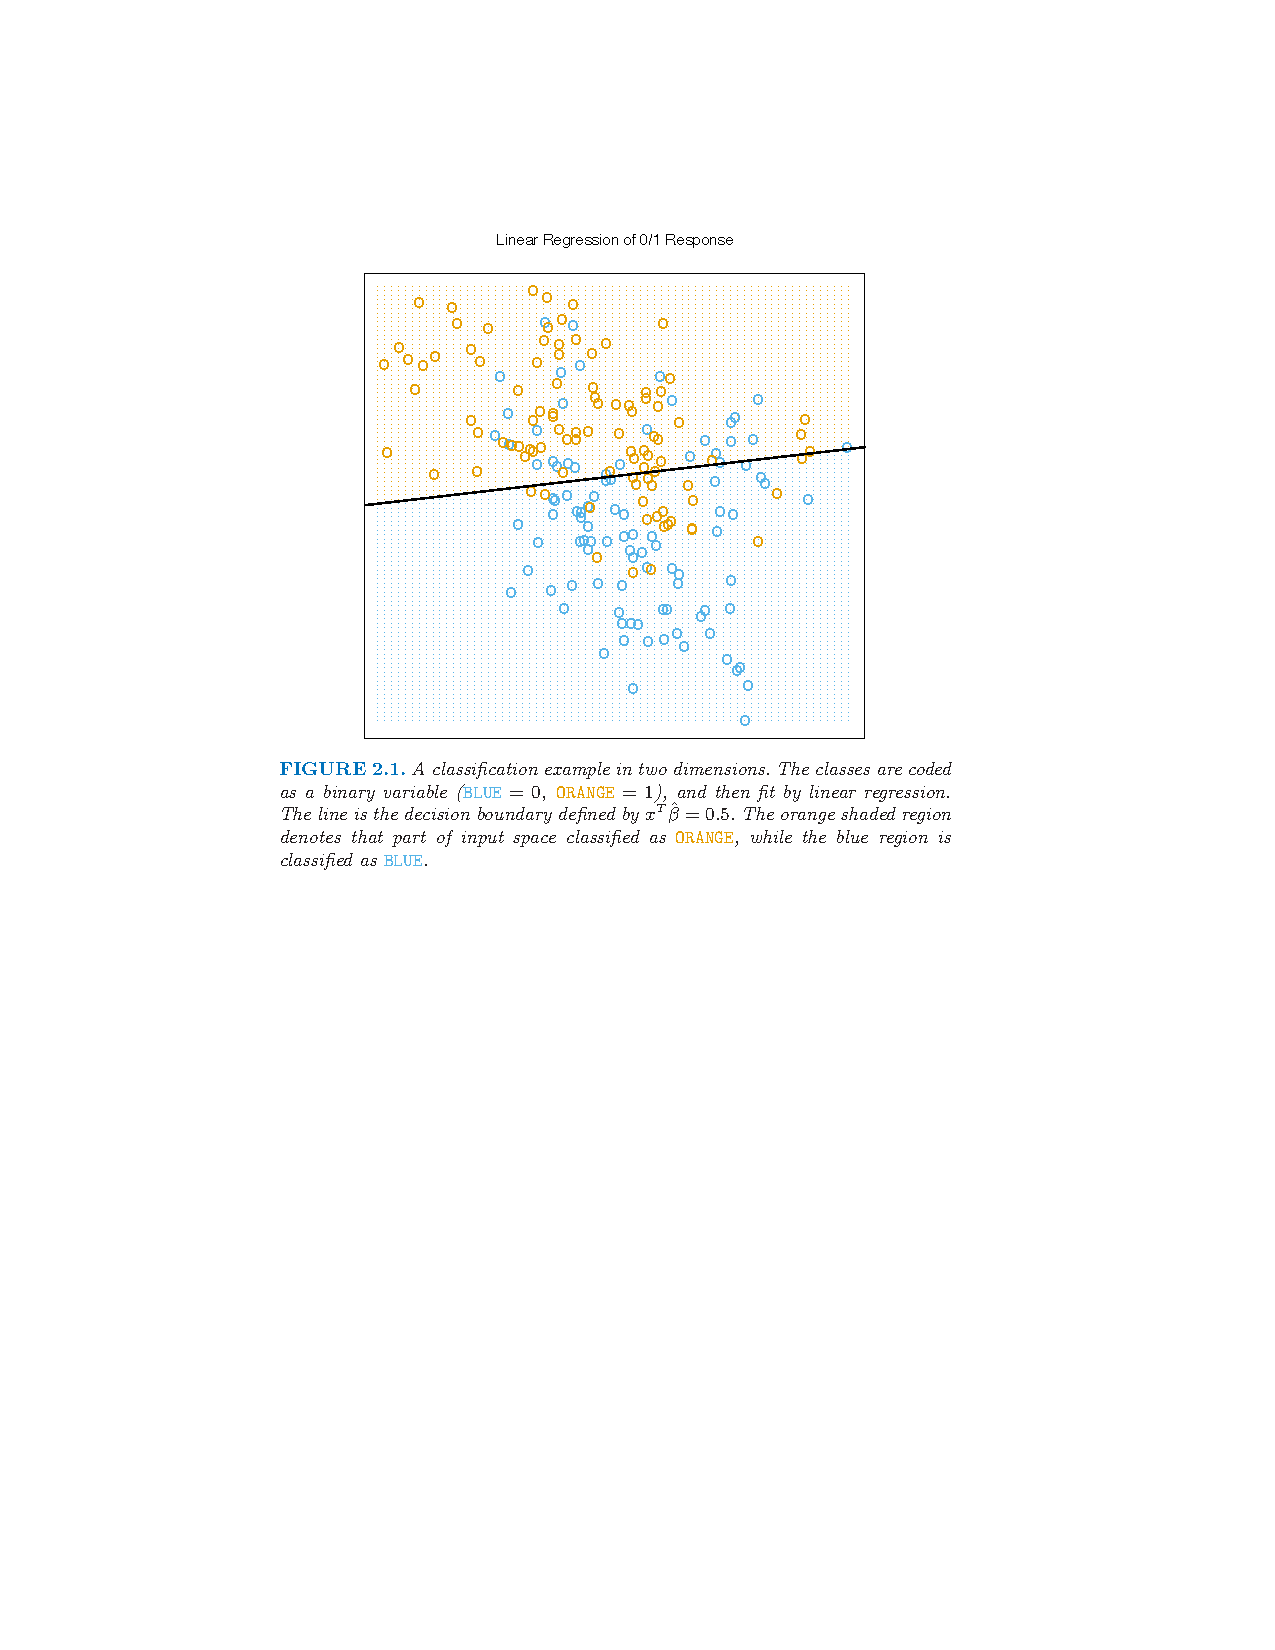
\includegraphics[height=0.9\textheight]{./resources/classifierOLS.pdf}
\label{classOLS}
\end{center}
\end{figure}
\end{frame}


\begin{frame}{Alternative}
\begin{itemize}
\item Lots of potential alternatives to our decision rule.
\item A simple idea is to hold a majority vote of neighboring points 
\begin{eqnarray*}
Y^{*} = \frac{1}{k} \sum_{x_i \in N_k(x)} y_i
\end{eqnarray*}
\item To avoid including ``yourself'' in your neighborhood, we often estimate on one sample and validate on another
\item How many parameters does this model have: None? One? $k$? 
\item Technically it has something like $N/k$.
\item As $N \rightarrow \infty$ this means we have an infinite number of parameters! (This is a defining characteristic of non-parametrics).
\end{itemize}
\end{frame}


\begin{frame}{15 Nearest Neighbor}
\begin{figure}[htbp]
\begin{center}
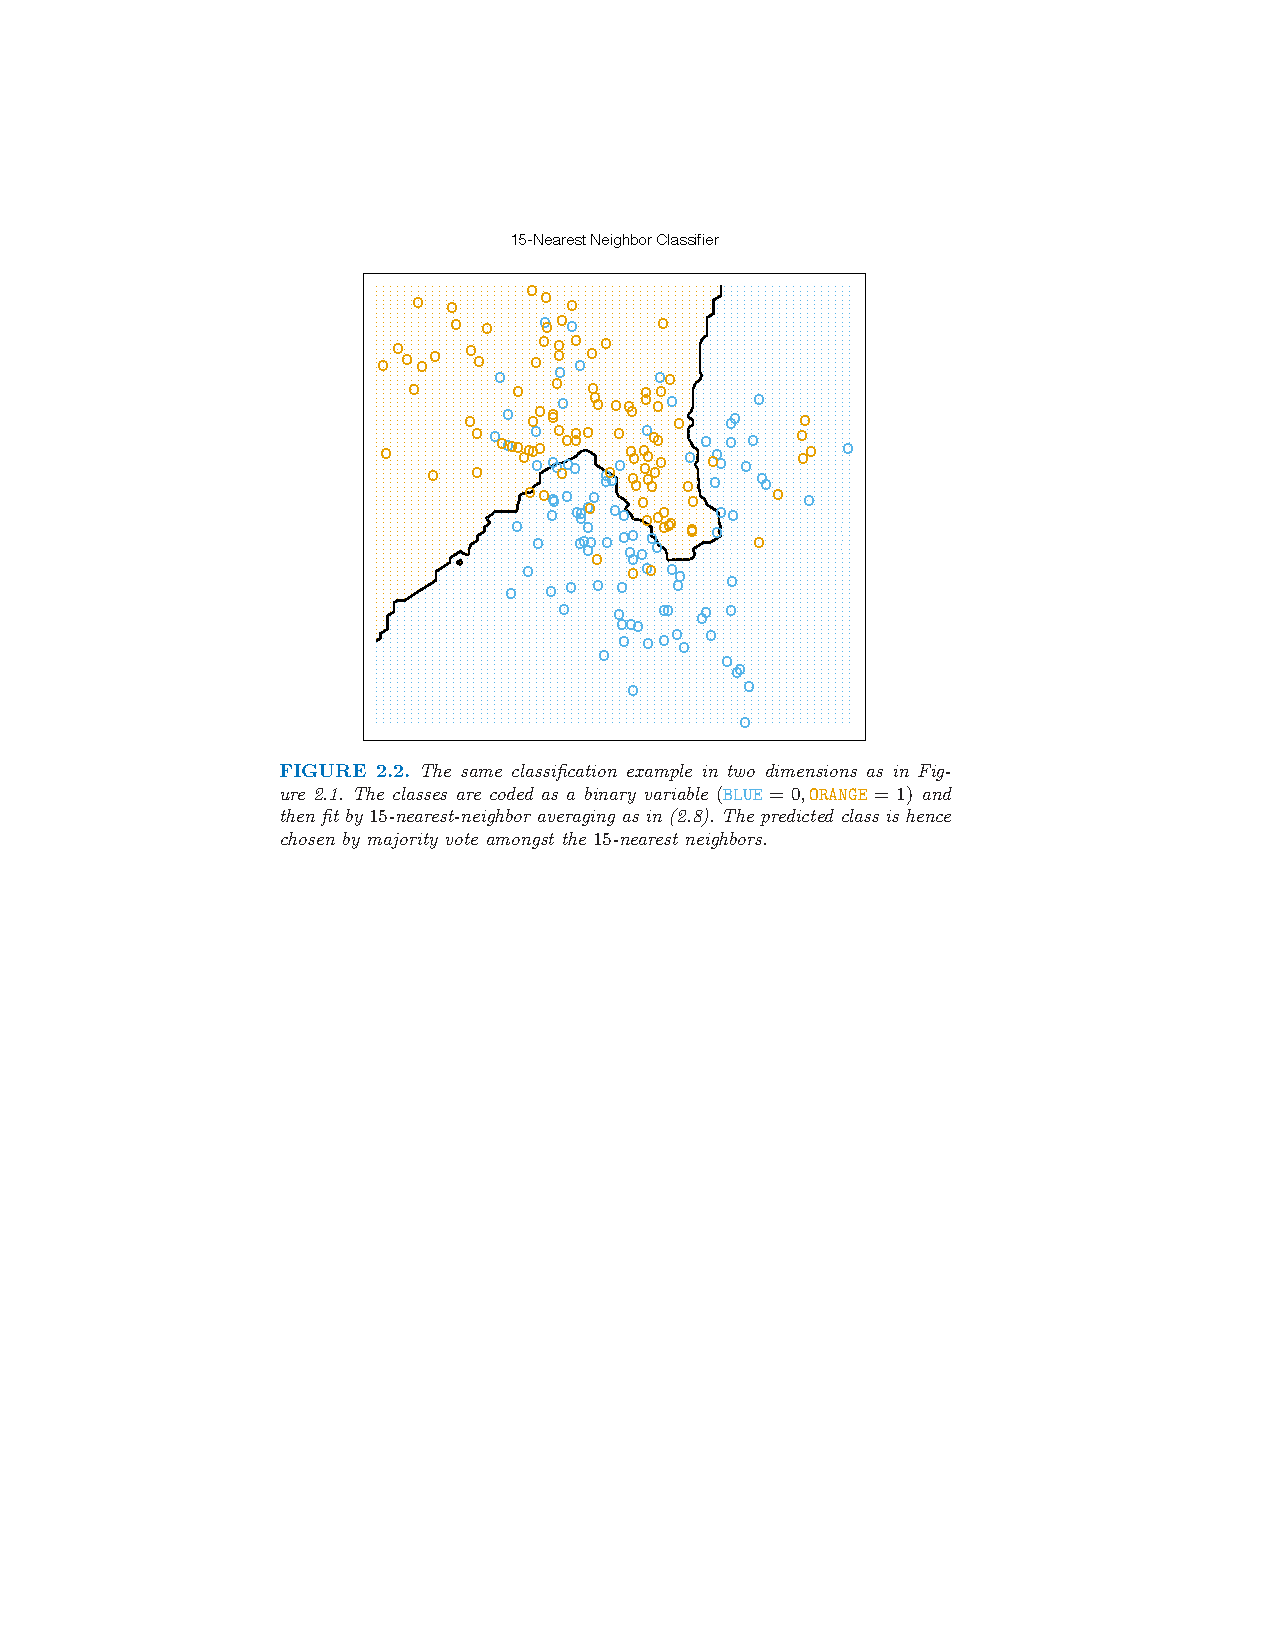
\includegraphics[height=0.95\textheight]{./resources/classifier15nn.pdf}
\label{class15nn}
\end{center}
\end{figure}
\end{frame}

\begin{frame}{Extreme: 1 Nearest Neighbor}
\begin{figure}[htbp]
\begin{center}
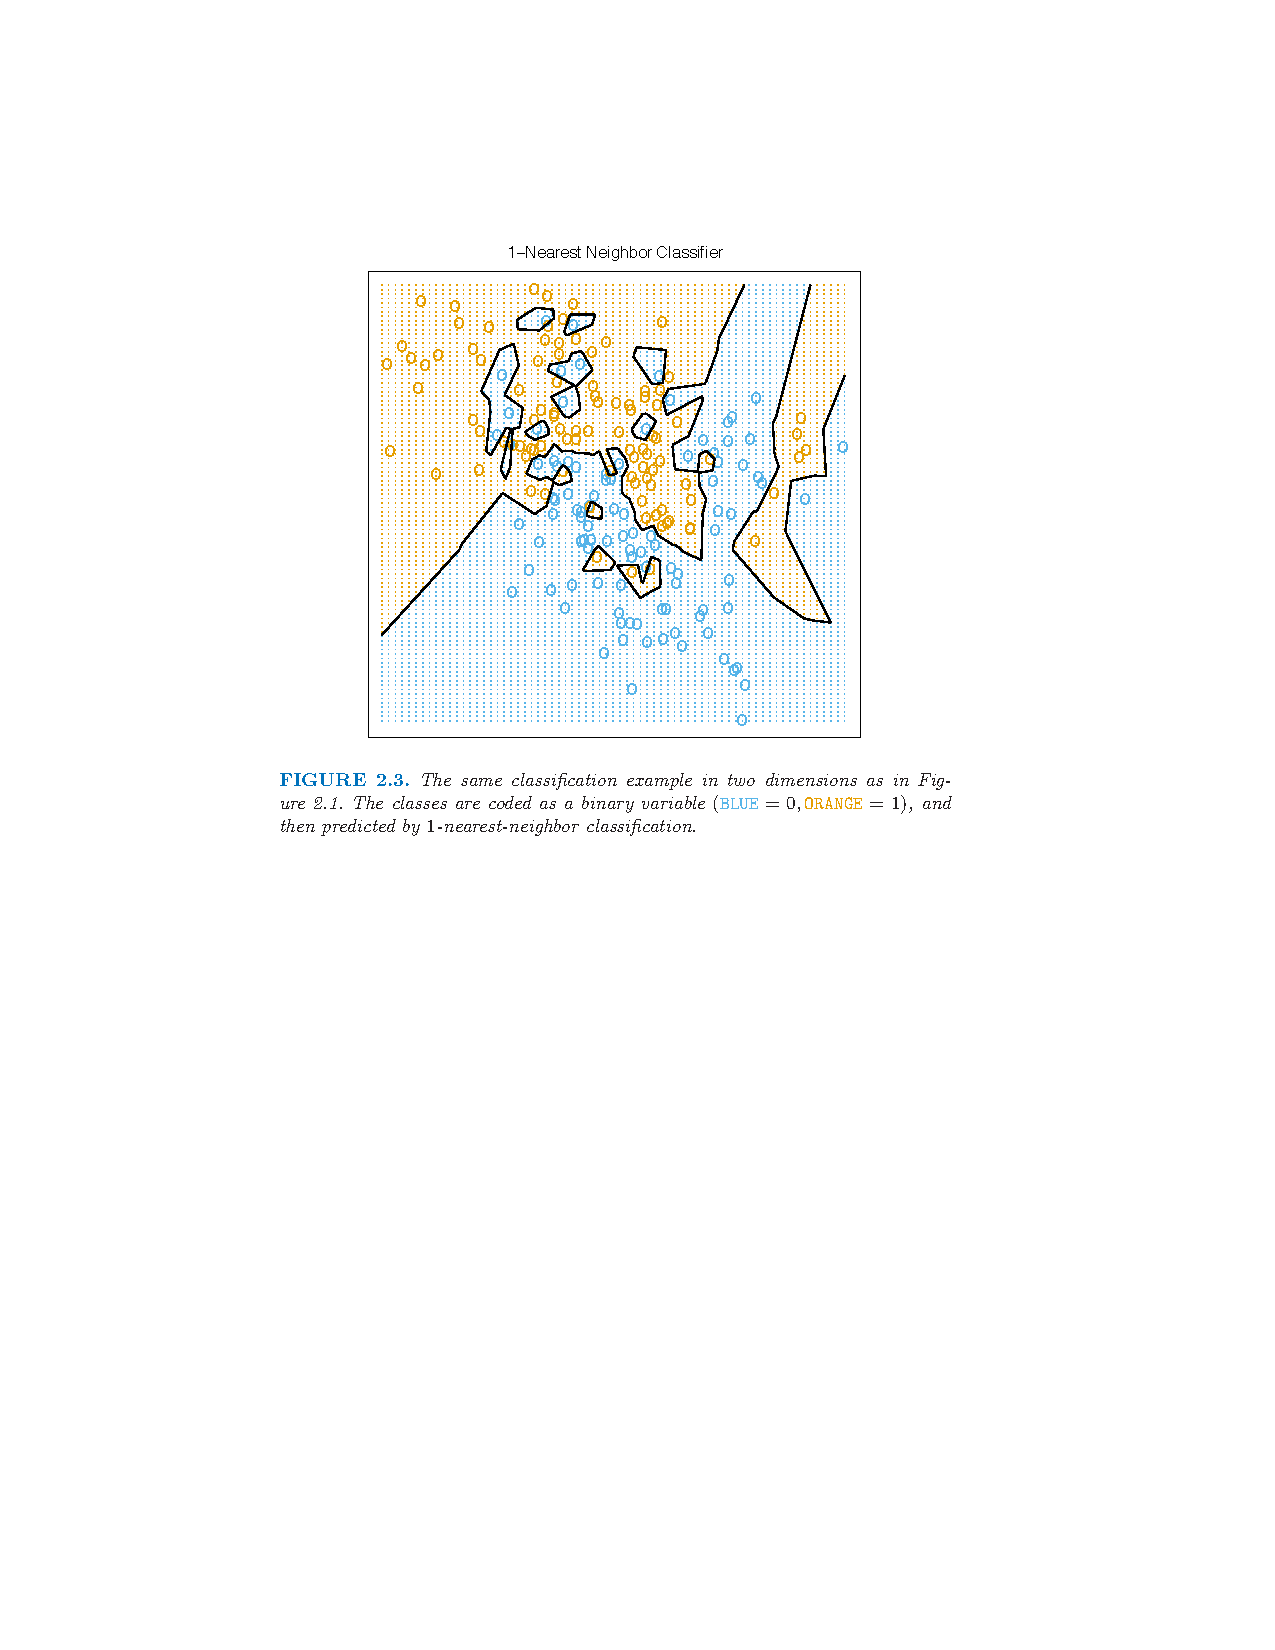
\includegraphics[height=0.95\textheight]{./resources/classifier1nn.pdf}
\label{class15nn}
\end{center}
\end{figure}
\end{frame}

\begin{frame}{Comparisons}
\begin{itemize}
\item What would happen if $K \rightarrow N$?
\item The k-NN model is locally constant.
\item The k-NN approach tends to be really bumpy which can be undesirable.
\end{itemize}
\end{frame}
\begin{frame}{What about?}
\begin{itemize}
\item If we fixed the fact that there are discrete jumps in who is in the neighborhood by smoothly weighting observations and varying those weights instead (Kernels).
\item Another drawback of $k-NN$ is that we consider distance in each $X$ dimension on the same scale, perhaps we could rescale the data to improve our ``closeness'' measure.
\item Instead of fitting a constant locally, we fit a linear function locally (Lowess).
\item Instead of using a global linear approximation in OLS use a more flexible nonlinear one.
\item There is a bias/variance tradeoff. \alert{explain}.
\end{itemize}
\end{frame}


\end{document}